\documentclass[12pt,a4paper]{IEEEtran}
\usepackage[latin1]{inputenc}
\usepackage{amsmath}
\usepackage{amsfonts}
\usepackage{amssymb}
\usepackage{graphicx}
\usepackage{float}
\usepackage{gensymb}
\usepackage{hyperref}
\usepackage{cite}
\usepackage[justification=centering, font={small,it}]{caption}
\author{Martin Tan (1002173), Leslie Tan (1002008), \\ Shoon Lei Khin (1002514), Cheryl Chan (1002478)}
\title{Physical World 1D Final Report}
\begin{document}

	\maketitle
	
	\section{Objectives}
	To incorporate the following design considerations in designing a cooling system for a thermoelectric cooler, in order to cool an aluminium block to 7 Degree Celsius in 5 minutes: \linebreak
	\begin{enumerate}
		\item Ensure effective cooling at the hot side of the Peltier chip, reducing delta T to increase the efficiency of the Peltier chip, with the use of forced air convection by fan.
		\item Insulate the cool side of the Peltier chip and attached aluminium block to reduce heat gain from surrounding.
	\end{enumerate}
	Our design includes a wind tunnel that directs the cold air from a fan attached to it towards the heat sink placed above the hot side of the Peltier chip. The heat sink is used to draw heat away from the hot side of the Peltier, together with the cold air directed by the wind tunnel. Additionally, the wind tunnel minimizes the change in air density, decreasing cross-sectional area and resulting in an increase in velocity. With that, cooling of the hot side of Peltier would increase, increasing the efficiency of the Peltier to cool the aluminium blocks within 5 minutes

	\section{Modelling the system with Python}
	Due to the complicated nature of the thermal system, a Python program was written to perform numerical analysis (Runge-Kutta Method) on the refrigerator to better predict the performance of the proposed design. (See attached Python file) It takes into account:
	\begin{enumerate}
		\item Heat capacity of the refrigerator's components, and hence varying temperatures of the hot and cold sides
		\item Conduction of heat through the refrigerator's components
		\item Conductive heat loss from the heat sink
		\item Current $I$ through the TEC as a function of $T_c$ and $T_h$
	\end{enumerate}\par
	\begin{figure}[H]
		\begin{center}
			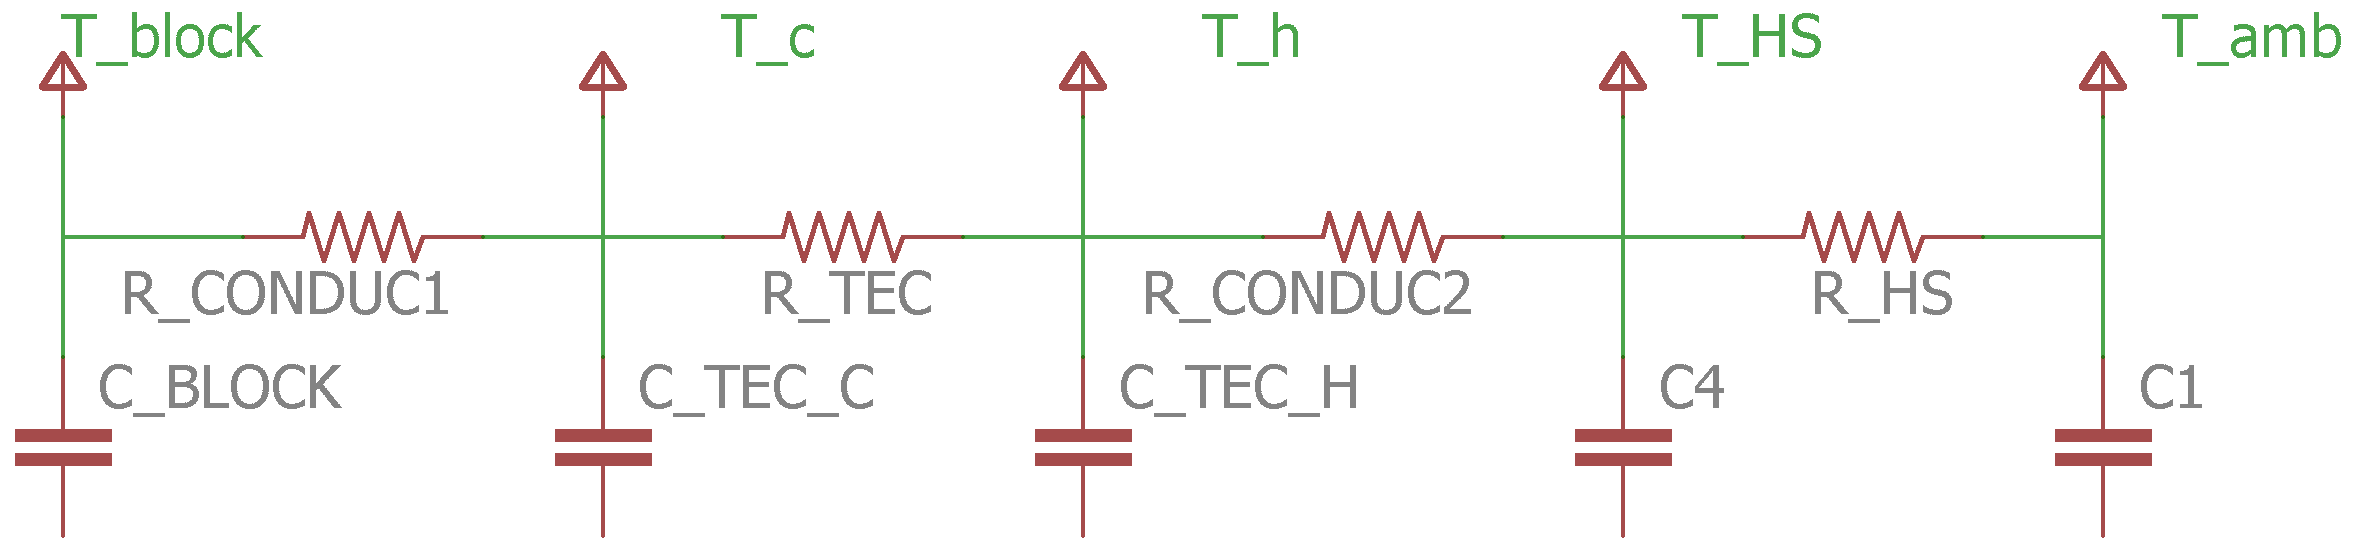
\includegraphics[width=0.5\textwidth]{thermal_circuit.png}
			\caption{Thermal Circuit Diagram of Refrigerator}
			\label{fig:thermalCurcuit}
		\end{center}
	\end{figure}
	Based on the thermal circuit diagram above, it can be seen that there are components in the system that have significant heat capacities. Furthermore, since there is a maximum voltage allowable, we cannot model the system as having a constant current. The current $I$ therefore is modelled as a function of $T_h$ and $T_c$, the other parameters being constant. Hence, the following equations were used to model the system.
	\begin{enumerate}
	\item $V=S_e (T_h-T_c )+IR \Rightarrow I = \frac{V-S_e(T_h-T_c)}{R}$
	\item $\dot{Q} = S_e I T_c - \frac{I^2R}{2} - \lambda (T_h - T_c)$
	\item $ \dot{Q} = mc\dot{T}$
	\end{enumerate}
	
	Simulations were ran for $0s \leq t \leq t_f$, with a discrete time step of $\frac{t_f}{100000}$, where $t_f = 300s$. with a time  It was found that it was possible to reach $7 \degree C$ within $78s$. The minimum temperature achieved after $300s$ is $3.20\degree C$. The maximum temperature reached by the hot side is $35.29 \degree C$. Below is a summary of the simulation parameters.
	
	\begin{table}[H]
		\centering
		\begin{tabular}{|l|l|}
			\hline
			Parameter                 & Value   \\ \hline
			Ambient Temp              & $298.15K$  \\ \hline
			Heat Sink Mass            & $0.045kg$ \\ \hline
			Heat Sink Surface Area    & $0.072m^2$ \\ \hline
			Air Velocity              & $0.4ms^-2$       \\ \hline
			Foam Insulation Thickness & $4mm$    \\ \hline
			Foam Thermal Conductivity & $0.045Wm^{-1}K^{-1}$        \\ \hline
			Mass of Aluminium Block   & $0.0294kg$        \\ \hline
			TEC Resistance            & $2.3\Omega$        \\ \hline
			TEC Seebeck Coefficient   & $0.042VK^{-1}$        \\ \hline
			TEC Thermal Conductance   & $0.52WK^{-1}$        \\ \hline
			TEC Applied Voltage       & $5.0V$        \\ \hline
		\end{tabular}
		\caption{Simulation Parameters}
		\label{simulationParameters}
	\end{table}
	
	\pagebreak
	Below is a graph of the cooling curve of the aluminium block for $0s \leq t \leq 300s$ illustrating the predicted performance of our system. It is observed that the initial cooling rate is large due to the non-zero capacity of the hot side; it takes some time for the hot side to heat up and for heat to conduct through the TEC back to the cold side.
	\begin{figure}[H]
		\begin{center}
			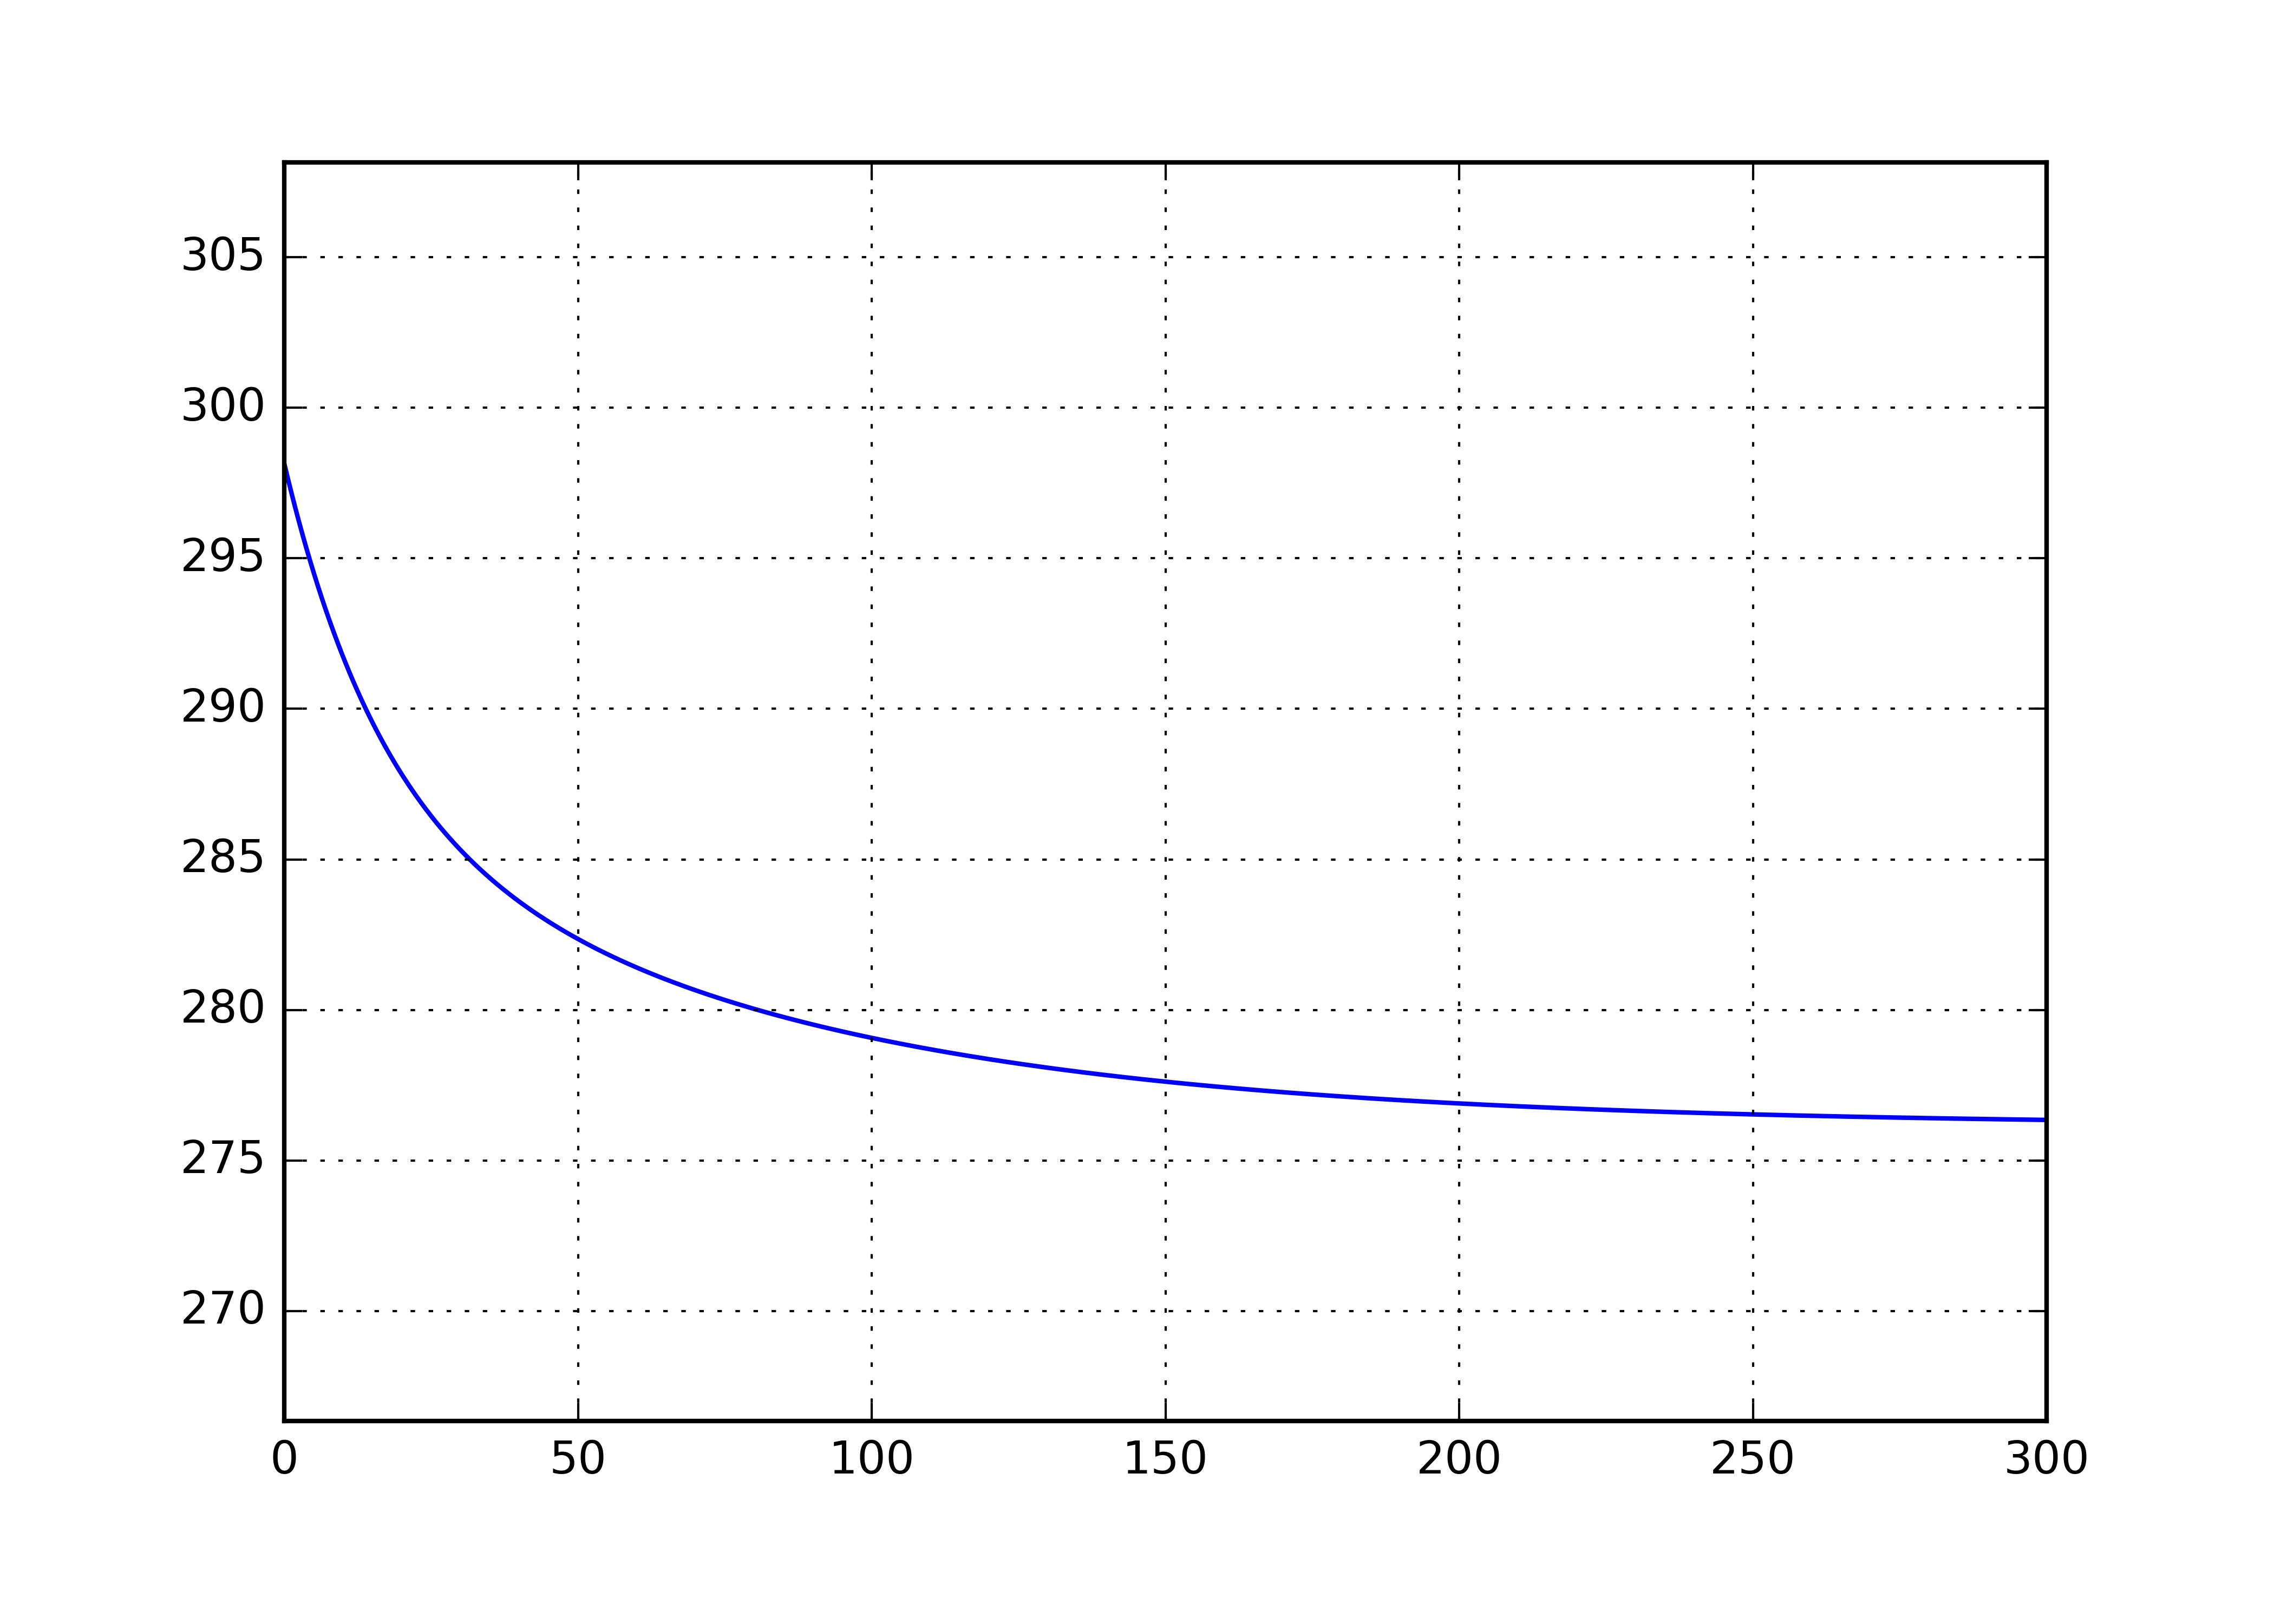
\includegraphics[width=0.4\textwidth]{T_c.png}
			\caption{Cooling curve: $T_c/K$ against Time/$s$}
			\label{fig:coolingcurve}
		\end{center}
	\end{figure}
	
	Below is a graph of the heating curve of the aluminium block for $0s \leq t \leq 300s$ illustrating that the temperature does not reach absolute maximum ratings of the TEC as specified in the datasheet. There is a maximum temperature reached, showing that initially, $\dot{Q}_h = \dot{Q}_c + \dot{W}$ is large, but once the cold side has cooled sufficiently and reached the minimum temperature, then $\dot{Q}_c = 0$, thus $T_h$ asymptotically reaches a steady state value of approximately $33\degree C$.
	\begin{figure}[H]
		\begin{center}
			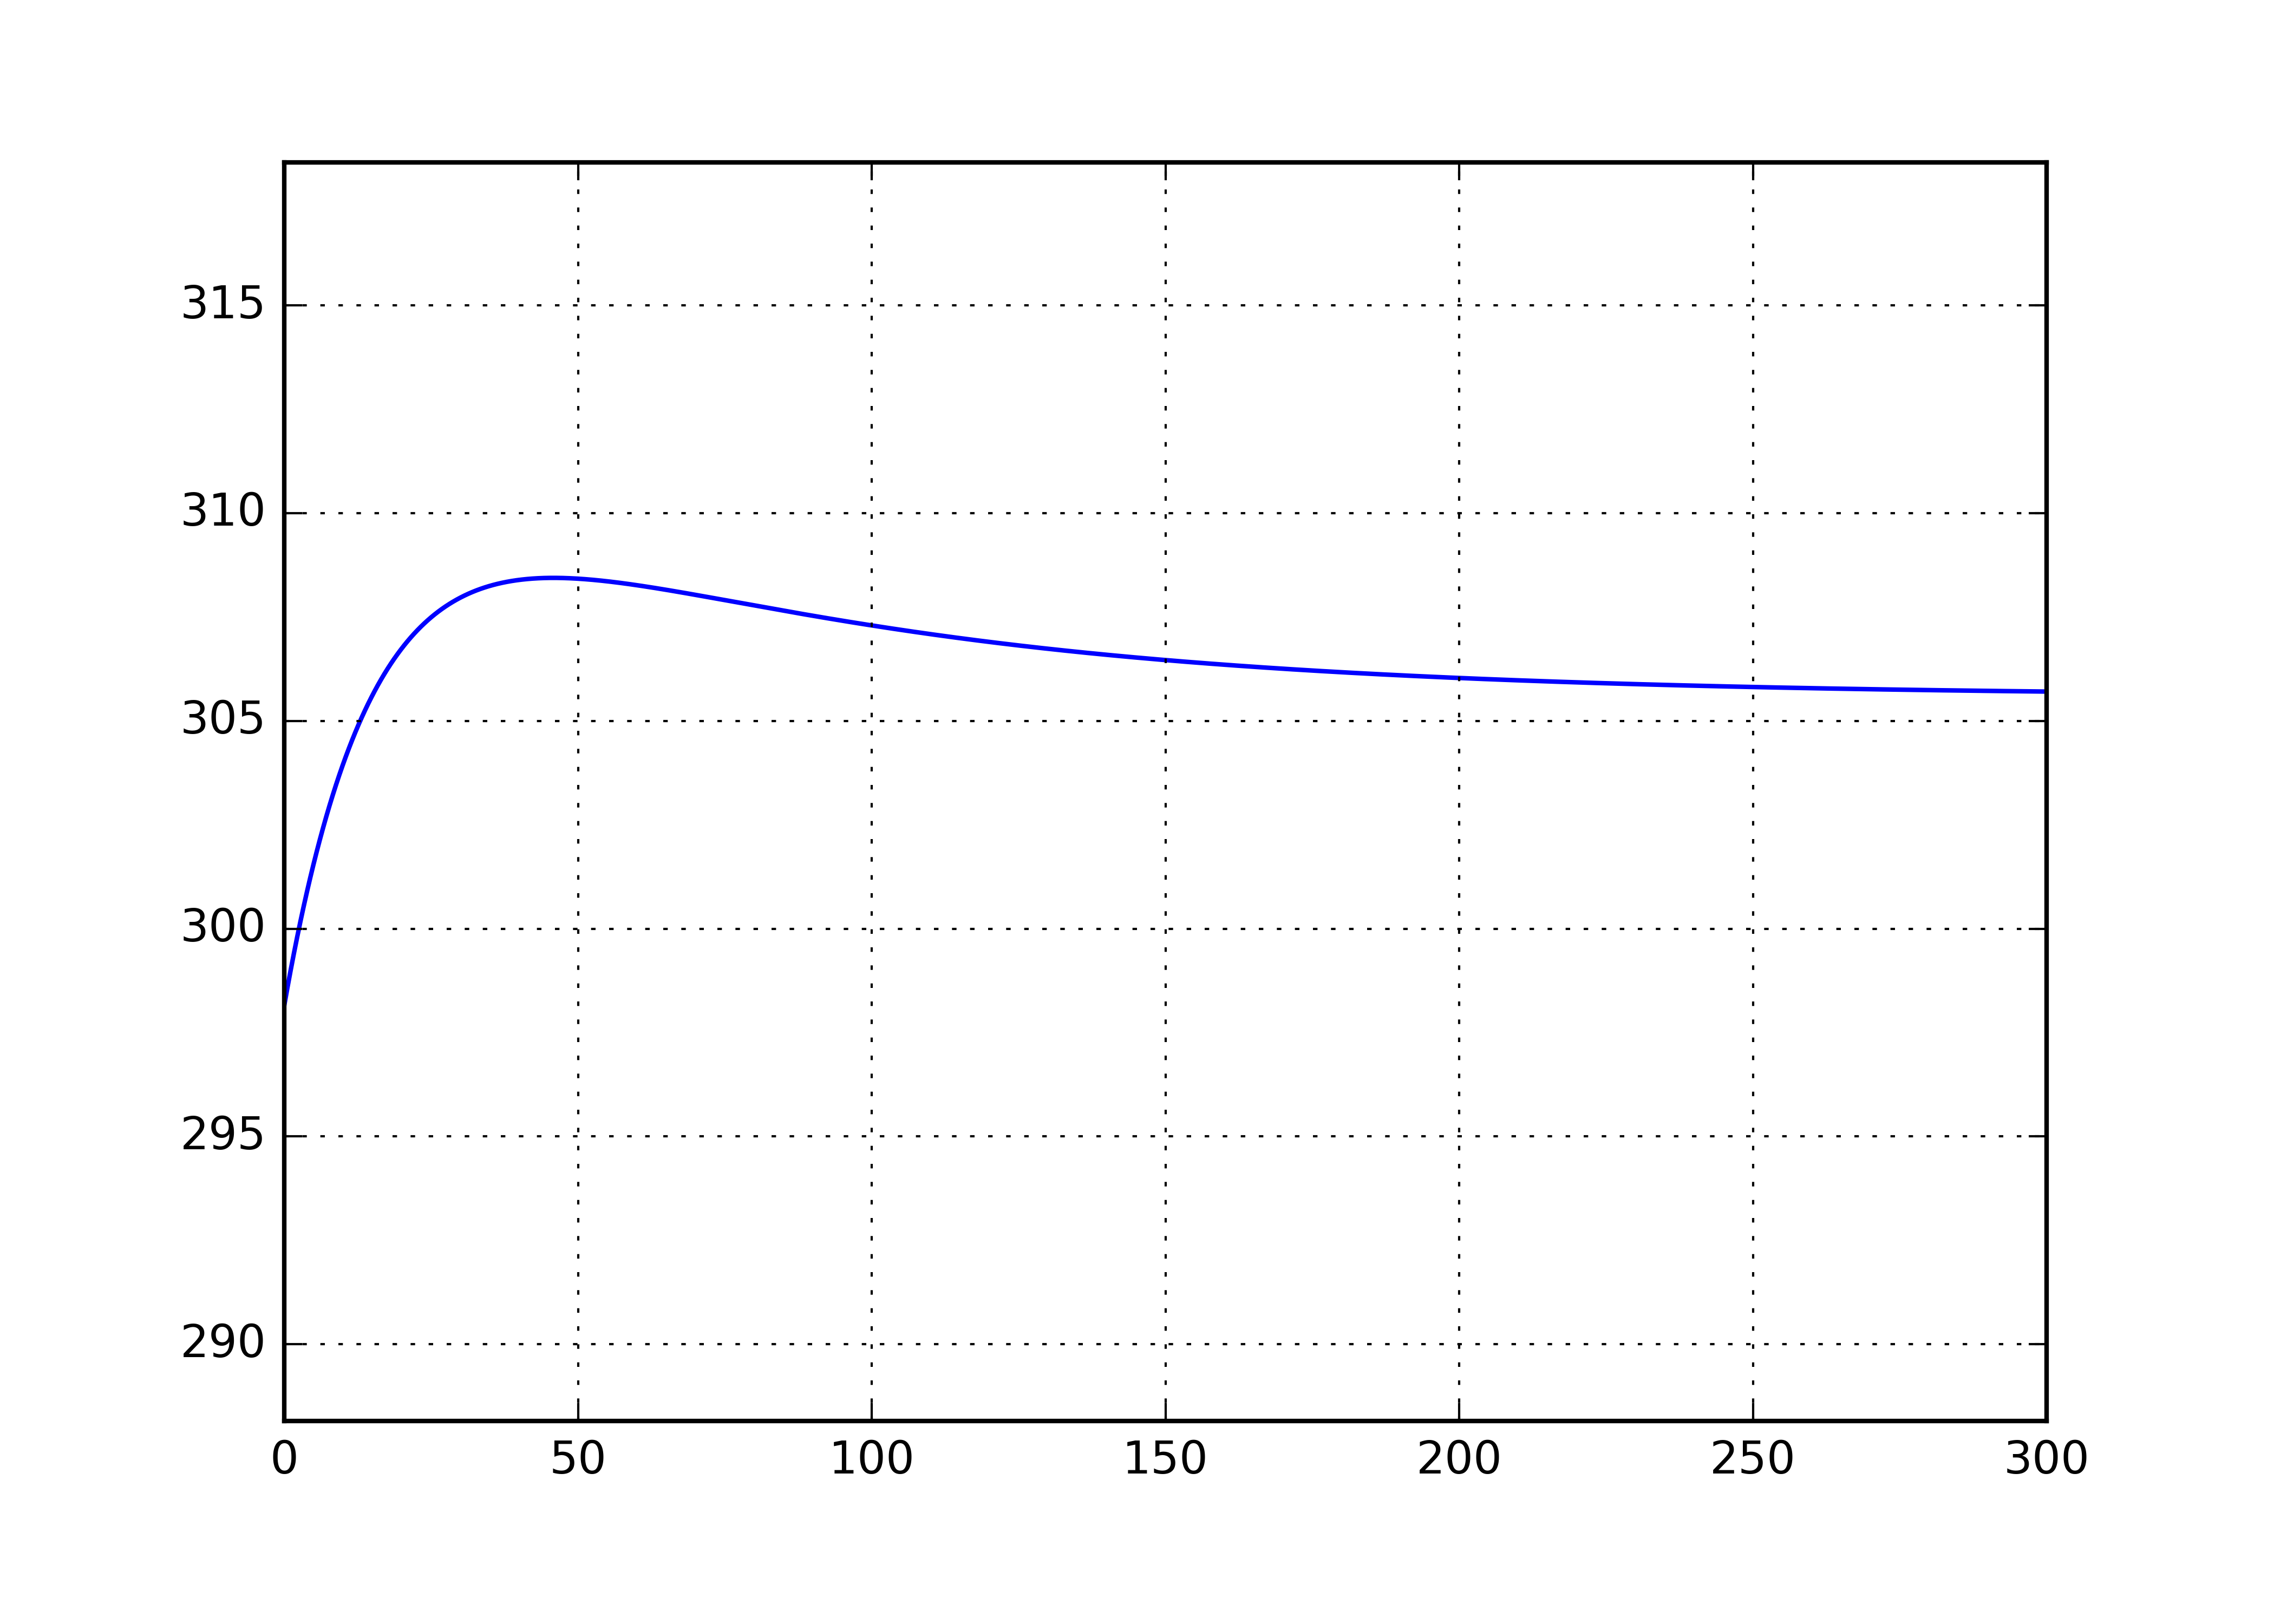
\includegraphics[width=0.4\textwidth]{T_h.png}
			\caption{Heating curve: $T_h/K$ against Time/$s$}
			\label{fig:heatingcurve}
		\end{center}
	\end{figure} \par

	\section{Design of Refrigerator}
	Based on the simulation that we carried out in Python, we designed a refrigerator according to or surpassing the parameters as specified in the simulation. A large aluminium heat sink with an approximate area of $720 cm^2$ was chosen.\linebreak
	
	A wind tunnel design was also chosen to increase the air mass flow rate over the aluminium heat sink. Our designed wind tunnel has an inlet area of $0.0144m^2$ and an outlet area of $0.002m^2$.\linebreak
	
	According to manufacturer specifications, the fan exit velocity is 2.5m/s when operated at 12V.  Assuming the fan is operating at 20\% power at 5V, our inlet velocity would thus be 0.5m/s.
	Mass Flow Rate, $\dot{m} = \rho AV = (1.184)(0.0144)(0.5) = 0.008525kg/s$, assuming density of air at $25\degree C$, $c = 1.184kg\cdot m^{-3}$, and no change to temperature inside wind tunnel (laminar flow).
	\linebreak
	$$\therefore V_{out} = \frac{\dot{m}}{\rho \cdot A_{out}} = \frac{0.008525}{(1.184)(0.002)} = 3.6m/s$$
	
	Based on our research (see references), the heat transfer coefficient of moving air $h$ can be estimated empirically by the equation:
	
	$$h = 10.45 - V_{air} + 10\sqrt{V_{air}}$$
	$$\therefore \dot{Q}_{Convection} = -hA(T_{H}-T_{Ambient})$$
	$$=(25.824)(0.072)(32-25)=13.02W$$	
	
	
	
	
	\newpage
	\section{Schematics of the Refrigerator Design}
	The diagram below shows the wind tunnel design chosen to increase mass flow rate of air over the heat sink.
	\begin{figure}[H]
		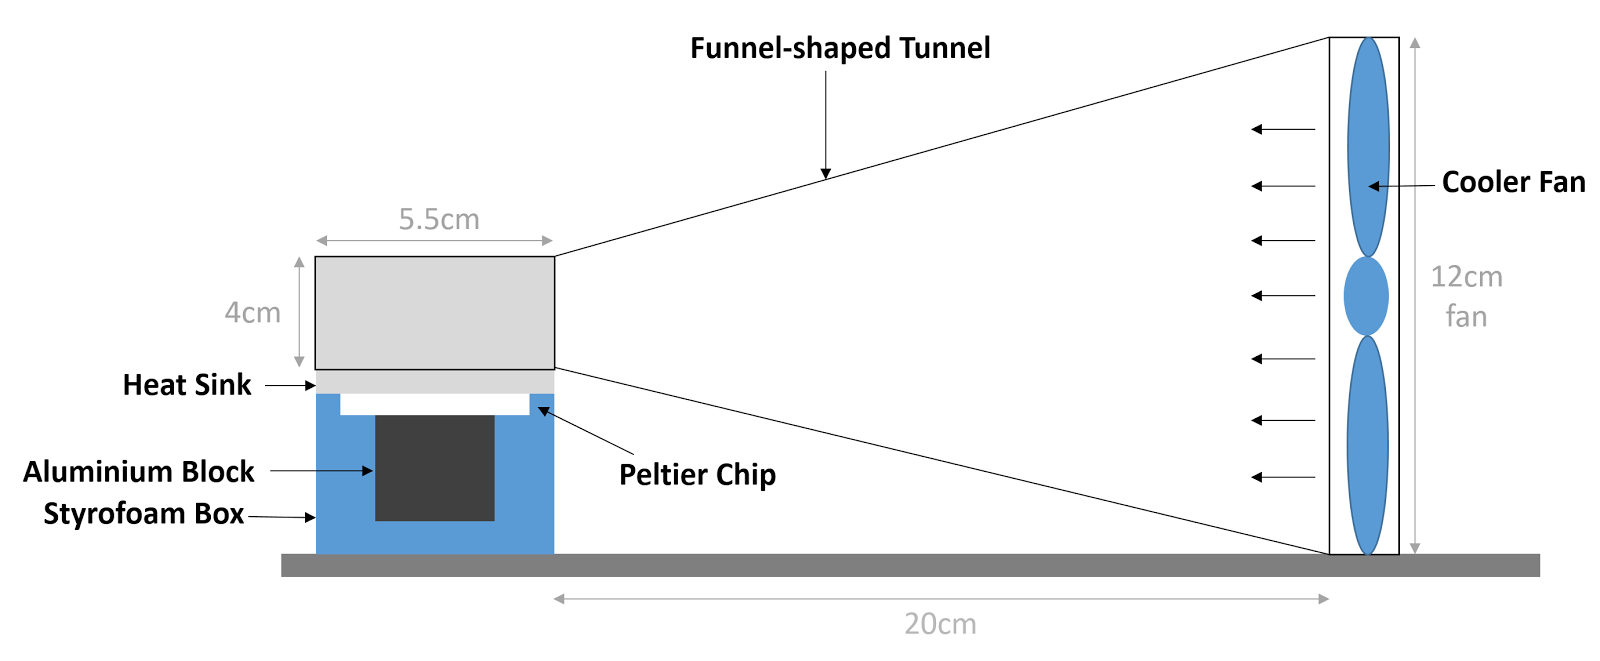
\includegraphics[width=0.5\textwidth]{tunnel_side_view.png}
		\begin{center}
			\caption{Heating curve: $T_h/K$ against Time/$s$}
			\label{fig:side_view}
		\end{center}
	\end{figure}
	\begin{figure}[H]
		\begin{center}
			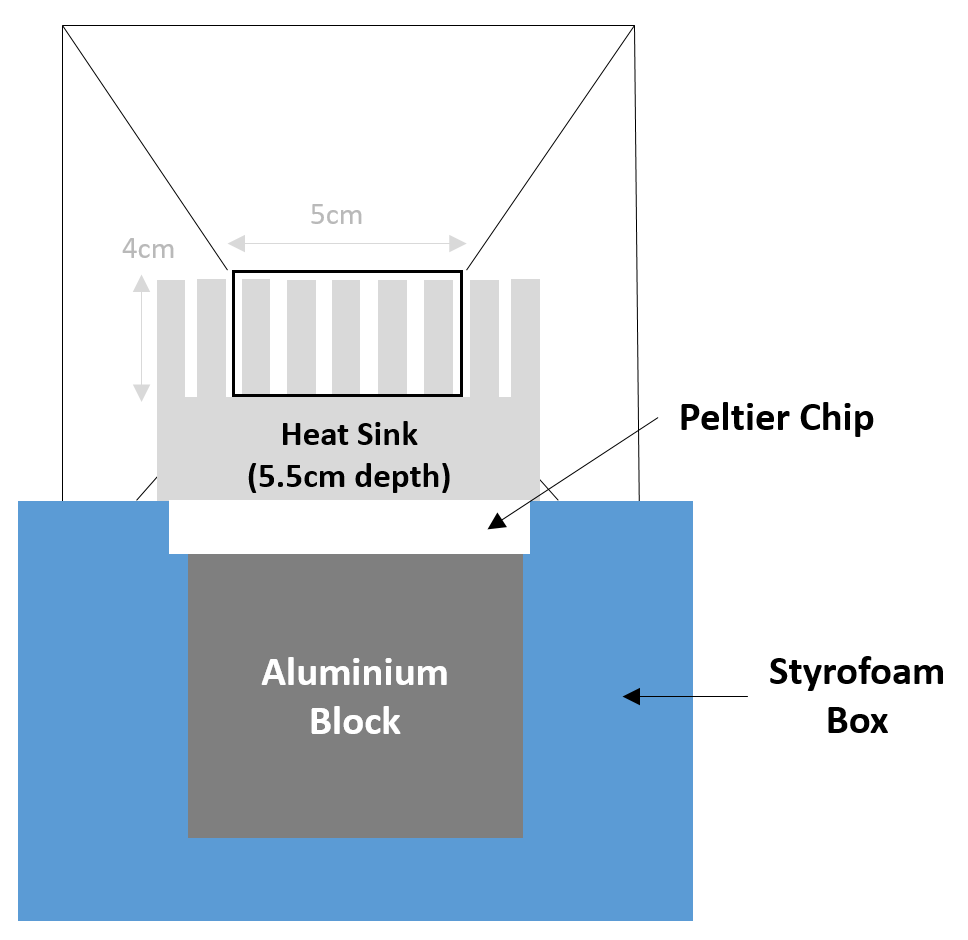
\includegraphics[width=0.5\textwidth]{cross_section_heatSink.png}
			\caption{Cross-section View of Nozzle and Heat Sink Fins}
			\label{fig:cross_section}
		\end{center}
	\end{figure} \pagebreak
	
	\section{Experimental Results}
	The graph below shows the graph of our experimental setup operating at $5V$ supply to the TEC. The final temperature attained at $t = 245s$ is $3.6\degree C$.
	\begin{figure}[H]
		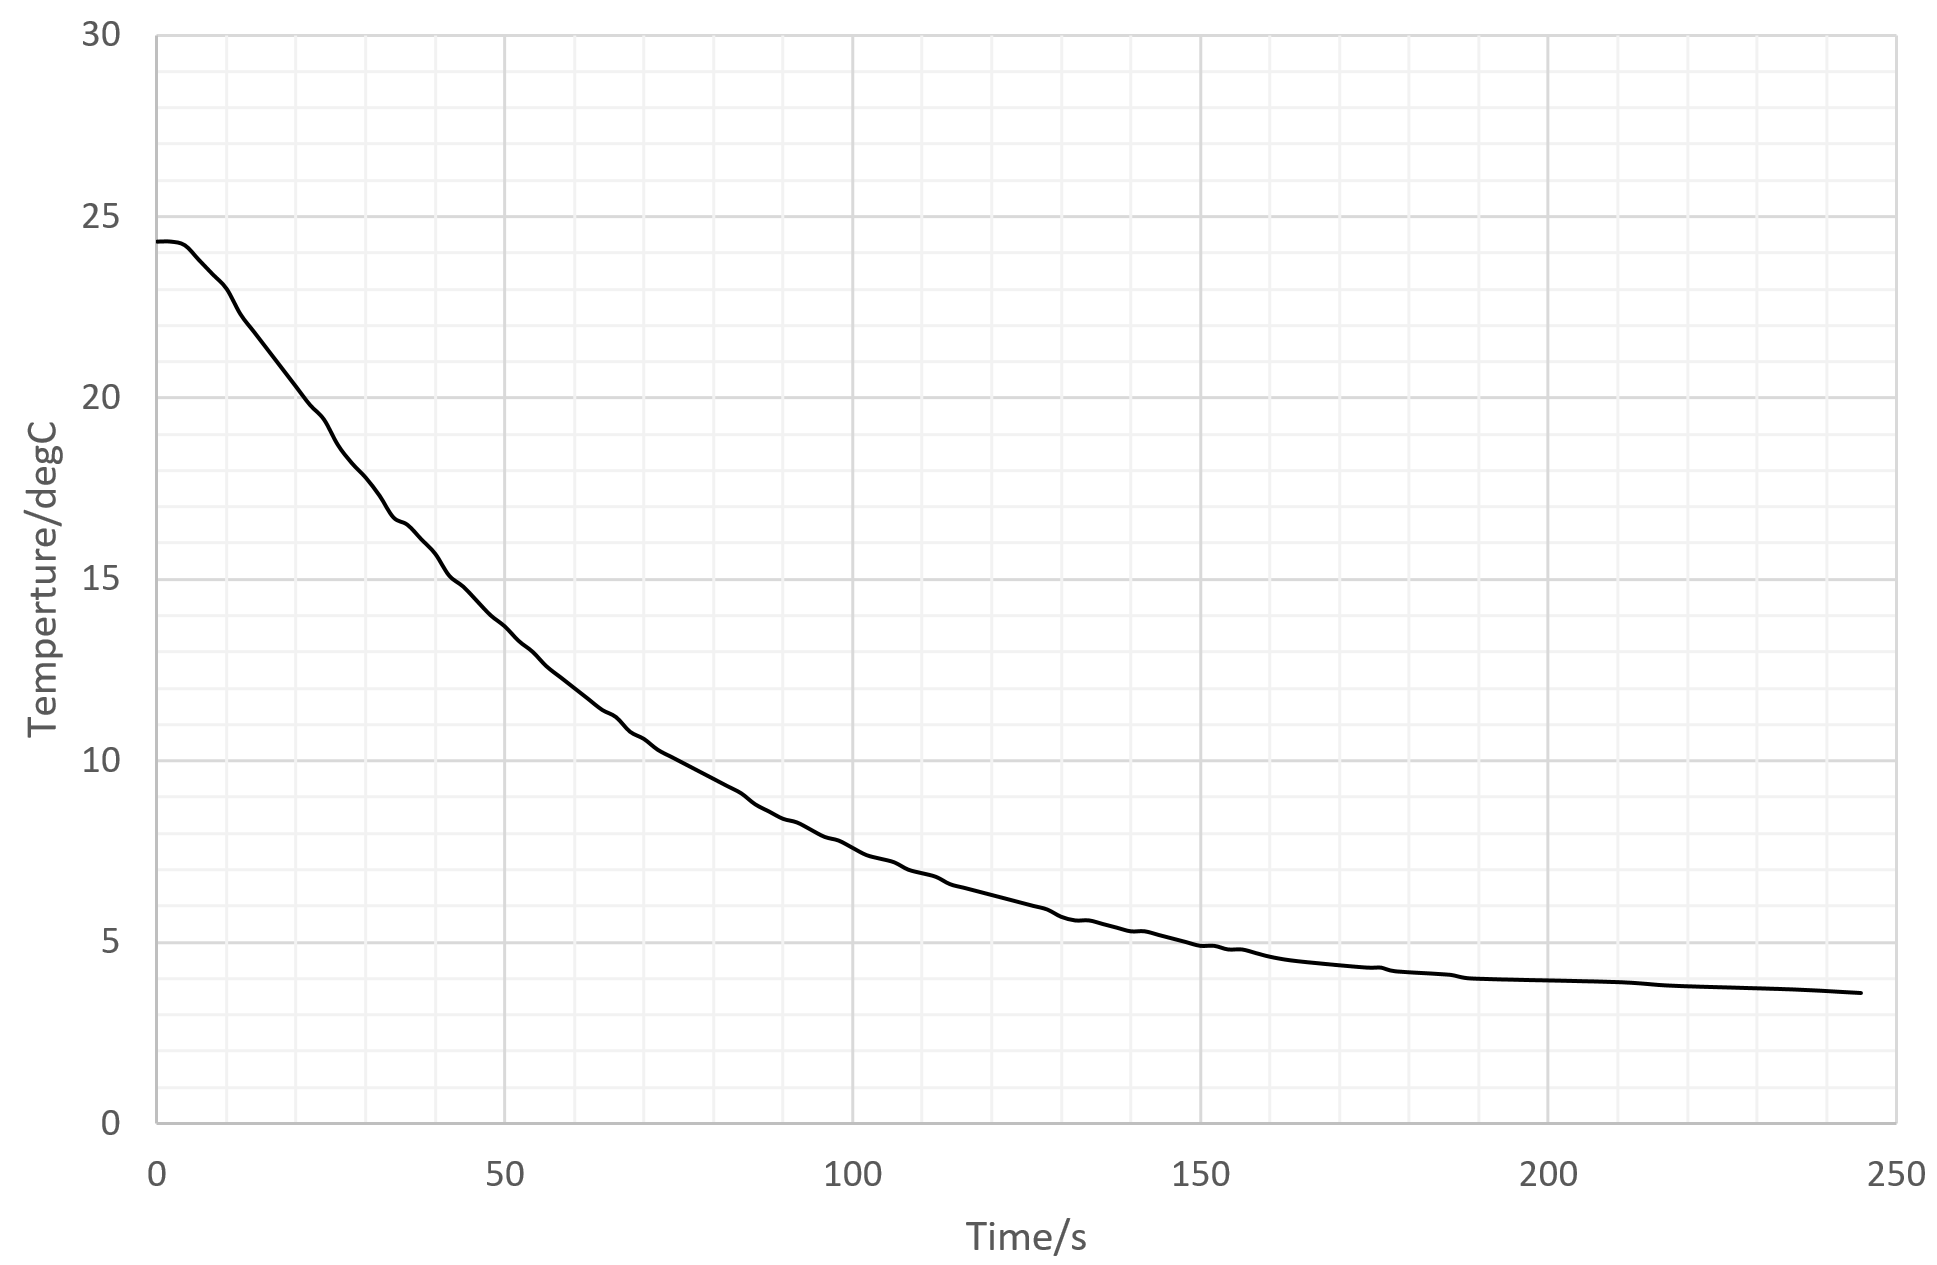
\includegraphics[width=0.5\textwidth]{cooling.png}
		\begin{center}
			\caption{Actual Cooling Curve: $T_c/\degree C$ against Time/$s$}
			\label{fig:cooling}
		\end{center}
	\end{figure}
	Based on the graph, the initial cooling rate is approximately $-0.21428Ks^{-1}$ which corresponds to $\dot{Q}_c = 0.0294kg \cdot 900Jkg^{-1}K^{-1} \cdot 0.21428Ks^{-1} = 5.67W$.
	This gives an initial Coefficient of performance $\frac{5.00V \cdot 2.04A}{5.67} = 1.79$
	\section{Results and Discussion}
	Based on our simulated estimate, the numerical analysis of the refrigerator shows significant correlation with our the empirical data, as the actual minimum temperature reached by our experiment is $3.6\degree C$, while the simulation predicts the final temperature to be $3.6\degree C$. \par
	
	However, the actual setup reached $7\degree C$ only at 108 seconds, whereas the simulation predicts the setup to reach $7\degree C$ in 78 seconds. This may perhaps be due to the incorrect predicted parameters of the TEC's electrical resistance, thermal conductance and Seebeck coefficient.
	
	\section{Youtube link of the video}
	\begin{center}
	\href{https://youtu.be/wcEqXpmNJk4}{https://youtu.be/wcEqXpmNJk4}
	\end{center}
	
	\section{References}
	http://www.engineeringtoolbox.com/convective-heat-transfer-d\textunderscore430.html
	
\end{document}